\chapter{Algebraic expressions}
\fancyfoot[LO,RE]{Focus Area: Mathematics}
\section{Rational and irrational numbers}
\setcounter{figure}{1}
\setcounter{subfigure}{1}

\nopagebreak
\label{m38348*cid2} $ \hspace{-5pt}\begin{array}{cccccccccccc}   
\includegraphics[width=0.75cm]{col11306.imgs/summary_video.png} &   \end{array} $ \hspace{2 pt}\raisebox{-5 pt}{} {(subsection shortcode: MG10033 )} \par 
\label{m38348*id62184}A number is a way of representing quantity. The numbers used in high school are all real numbers, but there are many different ways of writing any single real number.\par 
\label{m38348*id62191}This section describes rational and irrational numbers.\par \label{m38348*eip-195}
\setcounter{subfigure}{0}
\begin{figure}[H] % horizontal\label{m38348*circuits-1}
\textnormal{Khan Academy video on Integers and Rational Numbers}\vspace{.1in} \nopagebreak
\label{m38348*yt-media1}\label{m38348*yt-video1}
\raisebox{-5 pt}{ 
\includegraphics[width=0.5cm]{col11306.imgs/summary_www.png}} { (Video:  MG10034 )}
\vspace{2pt}
\vspace{.1in}
\end{figure}       

\par 
\subsection*{The big picture of numbers}
\addcontentsline{toc}{subsection}{The big picture of numbers}

\label{m38348*cid3} $ \hspace{-5pt}\begin{array}{cccccccccccc}   \end{array} $ \hspace{2 pt}\raisebox{-5 pt}{
\includegraphics[width=0.5cm]{col11306.imgs/summary_www.png}} {(subsection shortcode: MG10035 )} \par 
\label{m38348*id62547}
\setcounter{subfigure}{0}
\begin{figure}[H] % horizontal\label{m38348*id62548}
\begin{center}
\label{m38348*id62548!!!underscore!!!media}\label{m38348*id62548!!!underscore!!!printimage}
%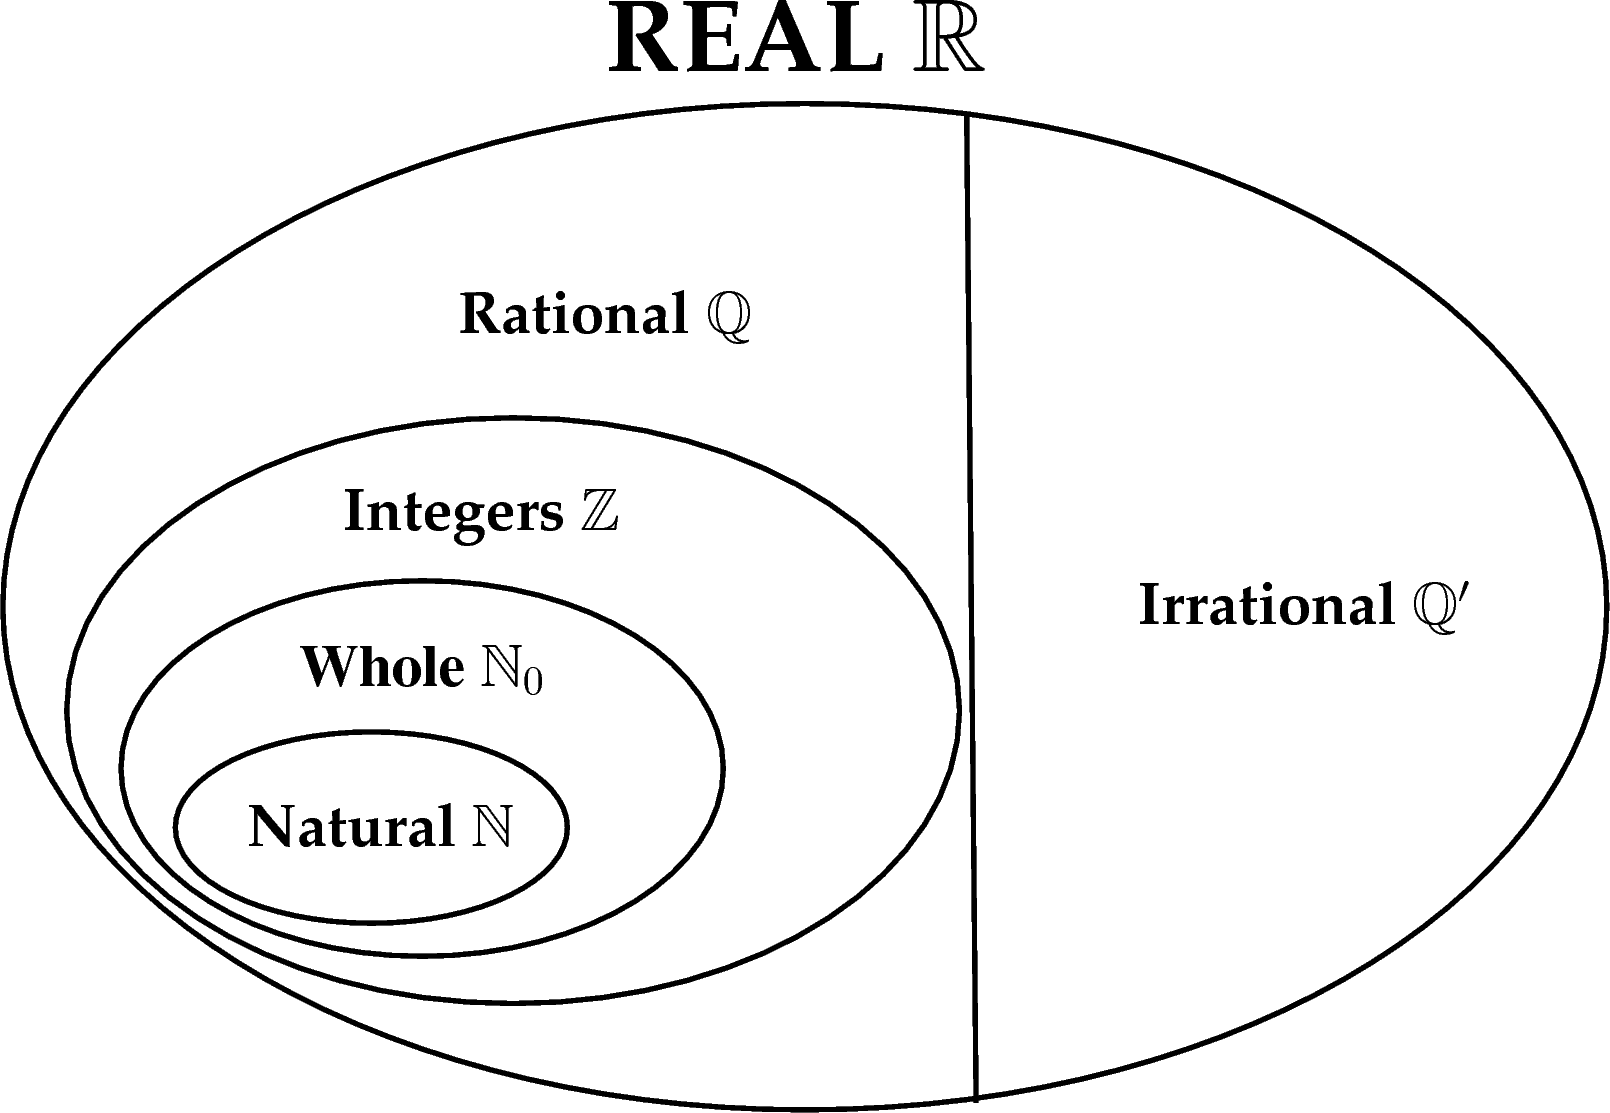
\includegraphics[width=9cm]{col11306.imgs/m38348_MG10C3_001.png} % m38348;MG10C3\_001.png;;;6.0;8.5;
\scalebox{0.6} % Change this value to rescale the drawing.
{
\begin{pspicture}(0,-4.764375)(14.481563,4.804375)
\psellipse[linewidth=0.04,dimen=outer](6.81,-0.484375)(6.81,4.28)
\psline[linewidth=0.04cm](8.18,3.695625)(8.26,-4.684375)
\psellipse[linewidth=0.04,dimen=outer](4.34,-1.364375)(3.8,2.5)
\psellipse[linewidth=0.04,dimen=outer](3.57,-1.854375)(2.57,1.61)
\usefont{T1}{ppl}{b}{n}
\rput(6.735781,4.350625){\Huge REAL $\mathbb{R}$}
\usefont{T1}{ppl}{b}{n}
\rput(11.03875,-0.484375){\Large Irrational $\mathbb{Q'}$}
\usefont{T1}{ppl}{b}{n}
\rput(5.11875,1.975625){\Large Rational $\mathbb{Q}$}
\usefont{T1}{ppl}{b}{n}
\rput(4.06875,0.275625){\Large Integers $\mathbb{Z}$}
\usefont{T1}{ppl}{b}{n}
\rput(3.21875,-2.324375){\Large Natural $\mathbb{N}$}
\psellipse[linewidth=0.04,dimen=outer](3.14,-2.354375)(1.68,0.83)
\usefont{T1}{ptm}{b}{n}
\rput(3.5735939,-1.024375){\Large Whole $\mathbb{N}_0$}
\end{pspicture} 
}
\vspace{2pt}
\vspace{.1in}
\end{center}
\end{figure}       
\par 
We use the following definitions:\par 
\label{m38348*id62559}\begin{itemize}[itemsep=5pt]
\label{m38348*uid1}\item natural numbers are $\{1; 2; 3; \ldots\}$
\label{m38348*uid2}\item whole numbers are $\{0; 1; 2; 3; \ldots\}$
\label{m38348*uid3}\item integers are $\{\ldots -3; -2; -1; 0; 1; 2; 3; \ldots\}$
\end{itemize}

\nopagebreak
\label{m38348*cid4} $ \hspace{-5pt}\begin{array}{cccccccccccc}   \end{array} $ \hspace{2 pt}\raisebox{-5 pt}{
\includegraphics[width=0.5cm]{col11306.imgs/summary_www.png}} {(subsection shortcode: MG10036 )} \par 

\Definition{Rational number}{
\label{m38348*id62709}A rational number is any number which can be written as: 
%       \label{m38348*uid6}\nopagebreak\noindent{}

\begin{equation*}
\frac{a}{b}
\end{equation*}
\label{m38348*id62732}where $a$ and $b$ are integers and $b\ne 0$. \par 
} 


\label{m38348*id62607}The following numbers are all rational numbers.\par 
\label{m38348*uid4}\nopagebreak\noindent{}

\begin{equation*}
\frac{10}{1};\frac{21}{7};\frac{-1}{-3};\frac{10}{20};\frac{-3}{6}
\end{equation*}
\label{m38348*id62687}We see that all denominators and all numerators are integers.\par 

\par
\label{m38348*id62778}This means that all integers are rational numbers, because they can be written with a denominator of 1.\par 
\label{m38348*id62782}Therefore consider

\begin{equation*}
\frac{\sqrt{2}}{7} ; \frac{20}{\pi}
\end{equation*}
\label{m38348*id62817}These are not rational numbers, because either the numerator or the denominator is not an integer.\par 
\label{m38348*id62829}A number may not be written as an integer divided by another integer, but may still
be a rational number. The rule is, if a number \textbf{can be} written
as a fraction of integers, it is rational even if it can be written in other
ways as well. These two examples might not look like rational numbers
at first glance, but because there have equivalent forms that can be expressed as an
integer divided by another integer, they are rational:\par 
\label{m38348*uid8}\nopagebreak\noindent{}
\begin{equation*}    
\frac{-1,33}{-3}=\frac{133}{300}; ~~~~~~\frac{-3}{6,39}=\frac{-300}{639}=\frac{-100}{213}
\end{equation*}
\label{m38348*secfhsst!!!underscore!!!id232}
% begin{exercise}   \subsubsubsection




\subsection*{Decimal numbers}
\addcontentsline{toc}{subsection}{Decimal numbers}
\nopagebreak
\label{m38348*cid5} $ \hspace{-5pt}\begin{array}{cccccccccccc}   \end{array} $ \hspace{2 pt}\raisebox{-5 pt}{
\includegraphics[width=0.5cm]{col11306.imgs/summary_www.png}} {(subsection shortcode: MG10037 )} \par 
\label{m38348*id63345}All integers and fractions with integer numerators and denominators are rational numbers. There are two more forms of rational numbers.\par 
\label{m38348*secfhsst!!!underscore!!!id245}



\begin{activity}{Decimal numbers }
\nopagebreak
\label{m38348*id63357}You can write the rational number
$\frac{1}{2}$ as the decimal number $0,5$. Write the following numbers as
decimals:\par 
\label{m38348*id63375}\begin{enumerate}[itemsep=5pt, label=\textbf{\arabic*}. ] 
\label{m38348*uid11}\item 
$\dfrac{1}{4}$
\label{m38348*uid12}\item 
$\dfrac{1}{10}$
\label{m38348*uid13}\item 
$\dfrac{2}{5}$
\label{m38348*uid14}\item 
$\dfrac{1}{100}$
\label{m38348*uid15}\item 
$\dfrac{2}{3}$
\end{enumerate}
\label{m38348*id63486}Do the numbers after the decimal comma end or do they continue? If they continue, is there a recurring pattern to the numbers? \par 
\end{activity}

\label{m38348*id63495}You can write any rational number as a decimal number but not all decimal numbers are rational numbers. However, two types of decimal numbers can be written as rational numbers:\par 
\label{m38348*id63500}\begin{itemize}
\label{m38348*uid16}\item decimal numbers that end or terminate, for example the fraction $\dfrac{4}{10}$ can be written as $0,4$.
\label{m38348*uid17}\item decimal numbers that have a recurring pattern of numbers, for example the fraction $\dfrac{1}{3}$ can be written as 
$0,\dot{3}$. 
The dot represents recurring $3$'s i.e.
$0,333\ldots=0,\dot{3}$.
\end{itemize}


\Tip{You can use a dot or a bar over the repeated numbers to indicate that the decimal is a recurring decimal.}
% 	\end{note}
% 	\end{minipage}
% 	\end{tabular}
\par

\subsection*{Converting terminating decimals into rational numbers}
\addcontentsline{toc}{subsection}{Converting terminating decimals into rational numbers}
A decimal number has an integer part and a fractional part. For example, $10,589$ has an integer part of $10$ and a fractional part of $0,589$ because $10+0,589=10,589$. The fractional part can be written as a rational number i.e. with a numerator and denominator that are integers. \\
\\
Each digit after the decimal point is a fraction with a denominator in increasing powers of $10$. For example 
\begin{itemize}
 \item $0,1$ is $\dfrac{1}{10}$
\item $0,01$ is $\dfrac{1}{100}$
\item $0,001$ is $\dfrac{1}{1000}$
\end{itemize}

This means that
\begin{equation*}
 \begin{array}{lll}10,589& = &10 + \dfrac{5}{10} + \dfrac{8}{100} + \dfrac{9}{1000} &\\ 
  &=& 10 \dfrac{589}{1000} \\
\\
&=& \dfrac{10589}{1000}
 \end{array}

\end{equation*}

\subsection*{Converting recurring decimals into rational numbers}

\label{m38348*cid7} $ \hspace{-5pt}\begin{array}{cccccccccccc}   \end{array} $ \hspace{2 pt}\raisebox{-5 pt}{
\includegraphics[width=0.5cm]{col11306.imgs/summary_www.png}} {(subsection shortcode: MG10039 )} \par 


\label{m38348*id63993}When the decimal is a recurring decimal, a bit more work is needed to write the fractional part of the decimal number as a fraction.\par 

\begin{wex}
{%title
Converting decimal numbers to fractions
}
{%question
\\
Write $0,\dot{3}$ in the form $\dfrac{a}{b}$ (where $a$ and $b$ are integers)
}
{%answer

\westep{Define an equation}
Let $x = 0,33333\ldots$


\westep{Multiply by $10$ on both sides}

$10x = 3,33333\ldots$


\westep{Subtract the first equation from the second equation}

$9x = 3 $

\westep{Simplify}

$ x = \dfrac{3}{9} = \dfrac{1}{3} $
}
\end{wex}


\begin{wex}
{%title
Converting decimal numbers to fractions
}
{%question
\\Write $5,\dot{4}\dot{3}\dot{2}$ as a rational fraction
}
{%answer

\westep{Define an equation}

$$ x = 5,432432432\ldots $$

\westep{Multiply by $1000$ on both sides}

$$ 1000x = 5432,432432432\ldots $$

\westep{Subtract the first equation from the second equation}

$$ 999x = 5427 $$

\westep{Simplify}

$$ x = \dfrac{5427}{999} = \dfrac{201}{37} $$

}
\end{wex}




\label{m38348*id64459}For the first example, the decimal was multiplied by $10$ and for the second example, the decimal was multiplied by $1000$. This is because for the first example there was only one digit (i.e. $3$) recurring, while for the second example there were three digits (i.e. $432$) recurring.\par 
\label{m38348*id64465}In general, if you have one digit recurring, then multiply by $10$. If you have two digits recurring, then multiply by $100$. If you have three digits recurring, then multiply by $1000$ and so on.\par

\label{m38348*id64474}Not all decimal numbers can be written as rational numbers. Why? Irrational decimal numbers like 
$\sqrt{2}=1,4142135\ldots$
cannot be written with an integer numerator and denominator, because they do not have a pattern of recurring digits and they do not terminate. However, when possible, you should try to use rational numbers or fractions instead of decimals.
% \label{m38348*secfhsst!!!underscore!!!id606}




\section{Irrational numbers}
\setcounter{figure}{1}
\setcounter{subfigure}{1}
\label{m38349}
%     Introduction
\nopagebreak
\label{m38349*cid2} $ \hspace{-5pt}\begin{array}{cccccccccccc}   \end{array} $ \hspace{2 pt}\raisebox{-5 pt}{
\includegraphics[width=0.5cm]{col11306.imgs/summary_www.png}} {(subsection shortcode: MG10055 )} \par 
\label{m38349*id324260}We have seen that recurring decimals may take a lot of paper and ink to write out. Writing numbers to many decimal places or a high accuracy is very inconvenient and rarely gives practical answers. For this reason we often estimate the number to a certain number of decimal places or to a given number of significant figures, which is even better.\par 
\Definition{Irrational numbers}{
\nopagebreak
%             \label{m38349*cid3} $ \hspace{-5pt}\begin{array}{cccccccccccc}   \end{array} $ \hspace{2 pt}\raisebox{-5 pt}{
\includegraphics[width=0.5cm]{col11306.imgs/summary_www.png}} {(subsection shortcode: MG10056 )} \par \label{m38349*id324624}
Irrational numbers are numbers that cannot be written as a fraction with the numerator and denominator as integers. This means that any number that is not a terminating or recurring decimal number is irrational. 

}

Examples of irrational numbers:\par 
%       \label{m38349*id324635}\nopagebreak\noindent{}

\begin{equation*}
\sqrt{2};~\sqrt{3};~\sqrt[3]{4};~\pi ;
~\frac{1+\sqrt{5}}{2}\approx 1,618
\end{equation*}


\label{m38349*notfhsst!!!underscore!!!id128}
% \begin{tabular}{cc}
% 	   \hspace*{-50pt}\raisebox{-8 mm}{ 
\includegraphics[width=0.5in]{col11306.imgs/pstip2.png}  }& 
% 	\begin{minipage}{0.85\textwidth}
% 	\begin{note}
\Tip{When irrational numbers are written in decimal form, they go on forever and
there is no repeated pattern of digits. \\The square roots of non-perfect squares and the cube roots of non-perfect cubes are all irrational.}
% 	\end{note}
% 	\end{minipage}
% 	\end{tabular}
\par
\label{m38349*id324739}If you are asked to identify whether a number is rational or irrational, first write the number in decimal form. If the number terminates then it is rational. If it goes on forever, then look for a repeated pattern of digits. If there is no repeated pattern, then the number is irrational.\par 
\label{m38349*id324745}When you write irrational numbers in decimal form, you may (if you have a lot of time and paper!) continue writing them for many, many decimal places. However, this is not convenient and it is often necessary to round off.\par 
\label{m38349*secfhsst!!!underscore!!!id133}


\begin{activity}{Irrational numbers }
\nopagebreak
\label{m38349*id324757}Which of the following cannot be
written as a rational number?\par \vspace{0.5cm}
\label{m38349*id324763}\textbf{Remember}: A rational number is a fraction with numerator and denominator as integers. Terminating decimal numbers or recurring decimal numbers are rational.\par 
\label{m38349*id324775}\begin{enumerate}[itemsep=5pt, label=\textbf{\arabic*}. ] 
\label{m38349*uid1}\item 
$\pi =3,14159265358979323846264338327950288419716939937510\ldots$
\label{m38349*uid2}\item $1,4$
\label{m38349*uid3}\item 
$1,618\phantom{\rule{0.166667em}{0ex}}033\phantom{\rule{0.166667em}{0ex}}989\phantom{\rule{0.166667em}{0ex}}\ldots$
\label{m38349*uid4}\item $100$
\item $1,7373737373\ldots$
\item $0,\overline{02}$
\end{enumerate}
\end{activity}


\begin{exercises}{}{
\nopagebreak
\label{m38348*id63121}\begin{enumerate}[itemsep=5pt, label=\textbf{\arabic*}. ] 
\label{m38348*uid9}\item If $a$ is an integer, $b$ is an integer and $c$ is irrational, which of the following are rational numbers? 
\label{m38348*id734}\begin{enumerate}[itemsep=5pt, label=\textbf{\alph*}. ] 
\item $\dfrac{5}{6}$\newline
\item $\dfrac{a}{3}$\newline
\item $\dfrac{-2}{b}$\newline
\item $\dfrac{1}{c}$\end{enumerate}
\label{m38348*uid10}\item If $\dfrac{a}{1}$ is a rational number, which of the following are valid values for $a$?\label{m38348*id7432}\begin{enumerate}[itemsep=5pt, label=\textbf{\alph*}. ] 
\item $1$\item $-10$\item $\sqrt{2}$\item $2,1$\end{enumerate}
%         \end{enumerate}
% \par \raisebox{-5 pt}{
\includegraphics[width=0.5cm]{col11306.imgs/summary_www.png}} Find the answers with the shortcodes:
%  \par \begin{tabular}[h]{cccccc}
%  (1.) l35  &  (2.) l3N  & \end{tabular}}
% \end{exercises}
% 
%            \begin{exercises}{Fractions }{
%             \nopagebreak
%       \label{m38348*id63882}\begin{enumerate}[itemsep=5pt, label=\textbf{\arabic*}. ] 
\label{m38348*uid20}\item Write the following as fractions:\label{m38348*id7322}
\begin{enumerate}[itemsep=5pt, label=\textbf{\alph*}. ] 
\item $0,1$\item $0,12$\item $0,58$\item $0,2589$
\end{enumerate}
%         \end{enumerate}
% \par \raisebox{-5 pt}{
\includegraphics[width=0.5cm]{col11306.imgs/summary_www.png}} Find the answers with the shortcodes:
%  \par \begin{tabular}[h]{cccccc}
%  (1.) l3R  & \end{tabular}}
% \end{exercises}
% 
% \begin{exercises}{Repeated Decimal Notation }{
% %             \nopagebreak
%       \label{m38348*id64513}\begin{enumerate}[itemsep=5pt, label=\textbf{\arabic*}. ] 
\label{m38348*uid23}\item Write the following using the recurring decimal notation:
\label{m38348*id64529}\begin{enumerate}[itemsep=5pt, label=\textbf{\alph*}. ] 
\label{m38348*uid24}\item $0,11111111\ldots$\label{m38348*uid25}\item $0,1212121212\ldots$\label{m38348*uid26}\item $0,123123123123\ldots$\label{m38348*uid27}\item $0,11414541454145\ldots$\end{enumerate}
\label{m38348*uid28}\item Write the following in decimal form, using the recurring decimal notation:
\label{m38348*id64650}\begin{enumerate}[itemsep=5pt, label=\textbf{\alph*}. ] 
\label{m38348*uid29}\item $\dfrac{2}{3}$\label{m38348*uid30}\item $1\dfrac{3}{11}$\label{m38348*uid31}\item $4\dfrac{5}{6}$\label{m38348*uid32}\item $2\dfrac{1}{9}$\end{enumerate}
\label{m38348*uid33}\item Write the following decimals in fractional form:
\label{m38348*id64767}\begin{enumerate}[itemsep=5pt, label=\textbf{\alph*}. ] 
\label{m38348*uid34}\item $0,\dot{5}$\label{m38348*uid35}\item $0,6\dot{3}$\label{m38348*uid36}\item $5,\overline{31}$\end{enumerate}
\end{enumerate}
% \par \raisebox{-5 pt}{
\includegraphics[width=0.5cm]{col11306.imgs/summary_www.png}} Find the answers with the shortcodes:
%  \par \begin{tabular}[h]{cccccc}
%  (1.) l3U  &  (2.) l3n  &  (3.) l3Q  & \end{tabular}}
\end{exercises}

\section{ Rounding off}
\nopagebreak
\label{m38349*cid4} $ \hspace{-5pt}\begin{array}{cccccccccccc}   
\includegraphics[width=0.75cm]{col11306.imgs/summary_fullmarks.png} &   \end{array} $ \hspace{2 pt}\raisebox{-5 pt}{} {(section shortcode: MG10057 )} \par 
\label{m38349*id324198}Rounding off or approximating a decimal number to a given number of decimal places is the quickest way to approximate a number. For example, if you wanted to round off $2,6525272$ to three decimal places, you would first count three places after the decimal and place a $|$ between the third and fourth numbers after the decimal.\par 
\label{m38349*id325085}\nopagebreak\noindent{}

\begin{equation*}
2,652|5272
\end{equation*}
\label{m38349*id325105}All numbers to the right of the $|$ are ignored after you have determined whether the number in the third decimal place must be rounded up or rounded down. You round u the final digit if the first digit after the $|$ was greater than or equal to $5$ and round down (leave the digit unchanged) otherwise. In the case that the first digit before the $|$ is $9$ and you need to round up, then the $9$ becomes a $0$ and the second digit before the $|$ is rounded up.\par 
\label{m38349*id325160}So, since the first digit after the $|$ is a 5, we must round up the digit in the third decimal place to a 3 and the final answer of $2,6525272$ rounded to three decimal places is $2,653$.
\par
\label{m38349*secfhsst!!!underscore!!!id199}\vspace{.5cm} 
\noindent
%       \hspace*{-30pt}
\includegraphics[width=0.5in]{col11306.imgs/pspencil2.png}   \raisebox{25mm}{   

\begin{wex}{Rounding-Off }
%       \label{m38349*probfhsst!!!underscore!!!id200}
%       \label{m38349*id325213}
{Round-off the following numbers to the indicated number of decimal places:\par 
\label{m38349*id325219}\begin{enumerate}[itemsep=5pt, label=\textbf{\arabic*}. ] 
%             \leftskip=20pt\rightskip=\leftskip\label{m38349*uid5}
\item $\frac{120}{99}=1,212121212\dot{1}\dot{2}$ to $3$ decimal places
\label{m38349*uid6}\item $\pi =3,141592654\ldots$ to $4$ decimal places
\label{m38349*uid7}\item $\sqrt{3}=1,7320508\ldots$ to $4$ decimal places
\label{m38349*uid789}\item $2,78974526\ldots$ to $3$ decimal places\end{enumerate}}
{
%       \vspace{5pt}
%       \label{m38349*solfhsst!!!underscore!!!id212}\noindent\textbf{Solution to Exercise } \label{m38349*listfhsst!!!underscore!!!id212}[itemsep=5pt, label=\textbf{Step} \textbf{\arabic*}. ] 
%             \leftskip=20pt\rightskip=\leftskip\item  
%       \label{m38349*id325360}[itemsep=5pt, label=\textbf{\alph*}. ] 
%             \leftskip=20pt\rightskip=\leftskip\label{m38349*uid8}

\westep{Mark off the required number of decimal places}

\begin{enumerate}[itemsep=5pt, label=\textbf{\arabic*}. ] 
\item  $\frac{120}{99}=1,212|121212\dot{1}\dot{2}$
%         \label{m38349*uid9}
\item           $\pi =3,1415|92654...$
%         \label{m38349*uid10}
\item           $\sqrt{3}=1,7320|508...$
\item $2,789|74526...$
\newline
\end{enumerate}
\westep{Check next digit to see if you must round up or round down}
\begin{enumerate}[itemsep=5pt, label=\textbf{\arabic*}. ]
%       \item  
%       \label{m38349*id325490}\begin{enumerate}[itemsep=5pt, label=\textbf{\alph*}. ] 
%             \leftskip=20pt\rightskip=\leftskip\label{m38349*uid11}
\item The last digit of $\frac{120}{99}=1,212|121212\dot{1}\dot{2}$  must be rounded down
\item The last digit of $\pi =3,1415|92654\ldots$ must be rounded up
\item The last digit of $\sqrt{3}=1,7320|508\ldots$ must be rounded up
\item  The last digit of $2,789|74526\ldots$ must be rounded up 
\newline Since this is a $9$, we replace it with a $0$ and round up the second last digit
\newline
\end{enumerate}
\westep{Write final answer}
\begin{enumerate}[itemsep=5pt, label=\textbf{\arabic*}. ]

%       \label{m38349*id325626}[itemsep=5pt, label=\textbf{\alph*}. ] 
%             \leftskip=20pt\rightskip=\leftskip\label{m38349*uid14}
\item $\frac{120}{99}=1,212$ rounded to $3$ decimal places
\item $\pi =3,1416$  rounded to $4$ decimal places
\item $\sqrt{3}=1,7321$ rounded to $4$ decimal places
\item $2,790$
\newline
\end{enumerate}

}  
\end{wex}

}

\begin{exercises}{}
{
Use your calculator to write the following in decimal form, round off to $3$ decimal places:
\begin{enumerate}[itemsep=5pt, label=\textbf{\arabic*}. ]
 \item $4\pi$
\item $\sqrt{11}$
\item $\dfrac{0,8}{3}$
\item $\sqrt[3]{7}$
\item $2\sqrt{10}$
\item $\dfrac{1}{18}$
\end{enumerate}

}
\end{exercises}


\section{Estimating surds}
\setcounter{figure}{1}
\setcounter{subfigure}{1}
\label{m38347}
%     \subsection{ Introduction}
\nopagebreak
\label{m38347*cid1} $ \hspace{-5pt}\begin{array}{cccccccccccc}   
\includegraphics[width=0.75cm]{col11306.imgs/summary_fullmarks.png} &   \end{array} $ \hspace{2 pt}\raisebox{-5 pt}{} {(subsection shortcode: MG10052 )} \par 
If the ${n}^{\mathrm{th}}$ root of a number cannot be simplified to a rational number, we call it a surd. For example, $\sqrt{2}$ and $\sqrt[3]{6}$ are surds, but $\sqrt{4}$ is not a surd because it can be simplified to the rational number $2$.\par 
In this chapter we will look at surds of the form $\sqrt[n]{a}$, where $a$ is any positive number, for example $\sqrt{7}$ or $\sqrt[3]{5}$. It is very common for $n$ to be $2$, so we usually do not write $\sqrt[2]{a}$. Instead we write the surd as just $\sqrt{a}$.\par 
\label{m38347*id258479}It is sometimes useful to know the approximate value of a surd without having to use a calculator. For example, we want to be able to estimate where a surd like $\sqrt{3}$ is on the number line. From a calculator we know that $\sqrt{3}$ is equal to $1,73205\ldots$. It is easy to see that $\sqrt{3}$ is above $1$ and below $2$. But to see this for other surds like $\sqrt{18}$ without using a calculator, you must first understand the following:\par 
\label{m38347*notfhsst!!!underscore!!!id71}
% \begin{tabular}{cc}
% 	\hspace*{-50pt}\raisebox{-8 mm}{\hspace{-0.2in}
\includegraphics[width=0.75in]{col11306.imgs/psfact2.png} } & 
% 	\begin{minipage}{0.85\textwidth}
% 	\begin{note}
\Identity{}{
\begin{center}
If $a$ and $b$ are positive whole numbers, and $a\lessthan{}b$, then $\sqrt[n]{a}\lessthan{}\sqrt[n]{b}$. 
\end{center}}
\par
%       
\Note{A perfect square is the number obtained when an integer is squared. For example $9$ is a perfect square since ${3}^{2}=9$. \\Similarly, a perfect cube is a number which is the cube of an integer. For example $27$ is a perfect cube, because ${3}^{3}=27$.}



\label{m38347*id259412}Consider the surd $\sqrt[3]{52}$, it lies somewhere between $3$ and $4$, because $\sqrt[3]{27}=3$ and $\sqrt[3]{64}=4$ and $52$ is between $27$ and $64$. Checking on a calculator we see that $\sqrt[3]{52}=3,73\ldots$ which is indeed between $3$ and $4$.\par 
\label{m38347*secfhsst!!!underscore!!!id162}\vspace{.5cm} 
\noindent
%       \hspace*{-30pt}
\includegraphics[width=0.5in]{col11306.imgs/pspencil2.png}   \raisebox{25mm}{   

\begin{wex}{ Estimating surds }{
%       \label{m38347*probfhsst!!!underscore!!!id163}
\label{m38347*id259741}Find the two consecutive integers such that $\sqrt{26}$ lies between them.\par 
\label{m38347*id259757}(Remember that consecutive numbers are two numbers that follow one another on the number line, for the set of integers. E.g.$5$ and $6$ or $8$ and $9$)  }
%       \vspace{5pt}
%       \label{m38347*solfhsst!!!underscore!!!id167}\noindent\textbf{Solution to Exercise } \label{m38347*listfhsst!!!underscore!!!id167}
{
% \begin{enumerate}[itemsep=5pt, label=\textbf{Step} \textbf{\arabic*}. ] 
%             \leftskip=20pt\rightskip=\leftskip\item  
\westep{Use perfect squares to guess the lower integer}     \label{m38347*id259781}${5}^{2}=25$. Therefore $5\lessthan{}\sqrt{26}$.\par 
%       \item  
\westep{Use perfect squares to guess the upper integer} \label{m38347*id259824} ${6}^{2}=36$. Therefore $\sqrt{26}\lessthan{}6$.\par 
%       \item  
\westep{The final answer is}\label{m38347*id259866} $5\lessthan{}\sqrt{26}\lessthan{}6$. \par 
%       \end{enumerate}
}
\end{wex}


\begin{wex}{Estimating surds }{
%       \label{m38347*probfhsst!!!underscore!!!id163}
Find the two consecutive integers such that $\sqrt[3]{49}$ lies between them.
}
{
\westep{Use perfect cubes to guess the lower integer}   ${3}^{3}=27$, therefore $3\lessthan{}\sqrt[3]{49}$.
%       \item  
\westep{Use perfect cubes to guess the upper integer} ${4}^{3}=64$, therefore $\sqrt[3]{49}\lessthan{}4$. 
%       \item  
\westep{So the answer is}
$3\lessthan{}\sqrt[3]{49}\lessthan{}4$

\westep{Check the answer by cubing all terms in the inequality and then simplify}\label{m38347*id259866} 
$27<49<64$. This is true so $\sqrt[3]{49}$ lies between $3$ and $4$.
%       \end{enumerate}
}
\end{wex}

\begin{exercises}{}
 {
Determine between which two consecutive integers the following numbers lie, without using a calculator:
\begin{enumerate}[itemsep=5pt, label=\textbf{\arabic*}. ]
\item $\sqrt{18}$
\item $\sqrt{29}$
\item $\sqrt[3]{5}$
\item $\sqrt[3]{79}$

\end{enumerate}

\end{exercises}



\section{Products}
\setcounter{figure}{1}
\setcounter{subfigure}{1}
\label{d4e6ddcad4e2d9e383c4732da6858c66}
%       Introduction and recap
\nopagebreak
\label{m39383} $ \hspace{-5pt}\begin{array}{cccccccccccc}   
\includegraphics[width=0.75cm]{col11306.imgs/summary_fullmarks.png} &   \end{array} $ \hspace{2 pt}\raisebox{-5 pt}{} {(section shortcode: MG10060 )} \par 
%   
\nopagebreak
\label{m39383*id267144}Mathematical expressions are just like sentences and their parts have special names. You should be familiar with the following words used to describe the parts of  mathematical expressions.\par 
\label{m39383*uid2}\nopagebreak\noindent{}

\begin{equation*}
3x^2 + 7xy -14 = 0
\end{equation*}



\begin{table}[H]
\begin{center}
\begin{tabular}{|l|l|}
\hline
\textbf{Name} & \textbf{Examples} \\
\hline
terms & $3x^2;~ 7xy;~ -14$\\ \hline
expression & $3x^2 + 7xy -14$\\ \hline
coefficient & $3;~7$\\ \hline
exponent & $2;~1$\\ \hline
base & $x;~y$\\ \hline
constant & $3;~7;-14$\\ \hline
variable & $x;~ y$\\ \hline
equation & $3x^2 + 7xy -14 = 0$\\ \hline
binomial & expression with two terms\\ \hline
trinomial & expression with three terms \\ \hline
\end{tabular}
\end{center}
\end{table} 

\par
\label{m39383*uid4}
\subsection*{Multiplying a monomial and a binomial}

\begin{wex}{Applying the distributive law}
{Write the following without brackets in its simplest form: $2a(a-1) - 3(a^{2}-1)$}
{
\westep{Apply the distributive law}
\begin{equation*}
 \begin{array}{lll} 2a(a-1) -3(a^{2}-1) &=& 2a(a) + 2a(-1) + (-3)(a^{2})+(-3)(-1) &
  &=& 2a^{2} - 2a - 3a^{2} + 3
 \end{array}
\end{equation*}

\westep{Simplify}
\begin{equation*}
 \begin{array}{lll} &=& -a^{2} -2a + 3 & 
 \end{array}
\end{equation*}


}


\end{wex}

\subsection*{Multiplying two binomials}
\addcontentsline{toc}{subsection}{Multiplying two binomials}
\nopagebreak
\label{m39383*id268015}A binomial is a mathematical expression with two terms, e.g. $ax+b$ and $cx+d$. If these two binomials are multiplied (or expanded) we get the following:
\label{m39383*id268064}\nopagebreak\noindent{}
\begin{equation*}
\begin{array}{ccc}\hfill (ax+b)(cx+d) & =& (ax)\left(cx\right)+\left(ax\right)d+b\left(cx\right)+bd\hfill  \\
& =& ac{x}^{2}+adx +bcx+bd\hfill\\
& =& ac{x}^{2}+x\left(ad+bc\right)+bd\hfill \end{array}
\end{equation*}

\Note{You may use FOIL = F(firsts) O(outers) I(inners) L(lasts) to remember this technique}
\par
\label{m39383*secfhsst!!!underscore!!!id342}\vspace{.5cm} 
\noindent
%       \hspace*{-30pt}
\includegraphics[width=0.5in]{col11306.imgs/pspencil2.png}   \raisebox{25mm}{   

\begin{wex}{Multiplying two binomials }{\label{m39383*probfhsst!!!underscore!!!id343}
\label{m39383*id268279}Find the product of $\left(3x-2\right)\mbox{ and }\left(5x+8\right)$ \par }{
%         \vspace{5pt}
%         \label{m39383*solfhsst!!!underscore!!!id346}\noindent\textbf{Solution to Exercise } \label{m39383*listfhsst!!!underscore!!!id346}[itemsep=5pt, label=\textbf{Step} \textbf{\arabic*}. ] 
\leftskip=20pt\rightskip=\leftskip\item  
\label{m39383*id268333}\nopagebreak\noindent{}

\begin{equation*}
\begin{array}{ccl}\hfill \left(3x-2\right)\left(5x+8\right)& =& \left(3x\right)\left(5x\right)+\left(3x\right)\left(8\right)+\left(-2\right)\left(5x\right)+\left(-2\right)\left(8\right)\hfill \\ & =& 15{x}^{2}+24x-10x-16\hfill \\ & =& 15{x}^{2}+14x-16\hfill \end{array}
\end{equation*}
}} 
\end{wex}


}
\noindent
\label{m39383*id268534}The product of two identical binomials is known as the square of the binomial and is written as:\par 
\label{m39383*id268543}\nopagebreak\noindent{}

\begin{equation*}
{\left(ax+b\right)}^{2}={a}^{2}{x}^{2}+2abx+{b}^{2}
\end{equation*}
\label{m39383*id268608}If the two terms are of the form $ax+b$\hspace{1ex}, and $ax-b$\hspace{1ex} then their product is:\par 
\label{m39383*id268642}\nopagebreak\noindent{}

\begin{align*}
\left(ax+b\right)\left(ax-b\right) &={a}^{2}{x}^{2}-{b}^{2} \\ &= (ax)^2-b^2
\end{align*}

\label{m39383*id268705}This product is known as the difference of two squares.\par 

\label{m39387*cid4}
\subsection*{ Multiplying a binomial and a trinomial}
\addcontentsline{toc}{subsection}{Multiplying a binomial and a trinomial}
\nopagebreak
\label{m39387*eip-109}
\setcounter{subfigure}{0}


\begin{figure}[H] % horizontal\label{m39387*productpolynomials}


\textnormal{Khan Academy video on products of polynomials.}\vspace{.1in} \nopagebreak
\label{m39387*yt-media1}\label{m39387*yt-video1}
\raisebox{-5 pt}{ 
\includegraphics[width=0.5cm]{col11306.imgs/summary_www.png}} { (Video:  MG10062 )}

\end{figure}   

\addtocounter{footnote}{-0}

A trinomial is a mathematical expression with three terms e.g. $ax^{2} + bx + c$.
Now we learn how to multiply a binomial and a
trinomial.\par 

\Tip{ \label{m39387*id271813}If the binomial is \begin{math}A+B\end{math} and the trinomial is \begin{math}C+D+E\end{math}, then the very first step is to apply the distributive law:\par 
\begin{equation*}
\left(A+B\right)\left(C+D+E\right)=A\left(C+D+E\right)+B\left(C+D+E\right)
\end{equation*}

If you remember this, you will never go wrong!\par }

\begin{wex}
{Multiplying a binomial and a trinomial 
}
{
Multiply \begin{math}x-1\end{math} with \begin{math}{x}^{2}-2x+1\end{math}.
} 
{
\westep{Apply the distributive law}
$
(x-1)(x^2-2x+1) &= x(x^2-2x+1)-1(x^2-2x+1)
$

\westep{Expand the bracket}

$
\phantom{(x-1)(x^2-2x+1) } = x^3-2x^2+x-x^2+2x-1
$

\westep{Simplify}

$
\phantom{(x-1)(x^2-2x+1) } = x^3-3x^2 + 3x1
$


}       

\end{wex}

}
\noindent

\label{m39387*secfhsst!!!underscore!!!id1562}\vspace{.5cm}

\begin{exercises}{}
Find the products of the following:

\begin{multicols}{2}
\begin{enumerate}[label=\textbf{\arabic*}., itemsep=5pt]
\item $2y(y+4)$ 
\item $(y+5)(y+2) $
\item $(2-t)(1-2t)$
\item $(x-4)(x+4)$
\item $ (2p+9)(3p+1)$
\item $(3k-2)(k+6)$
\item $(s+6)^2$
\item $-(7-x)(7+x)$
\item $(3x-1)(3x+1)$
\item $(7k+2)(3-2k)$
\item $(1-4x)^2$
\item $(-3-y)(5-y)$
\item $(8-x)(8+x)$
\item $(9+x)^2$
\item$\left(-2{y}^{2}-4y+11\right)\left(5y-12\right)$ 
\item$\left(7{y}^{2}-6y-8\right)\left(-2y+2\right)$% make-rowspan-placeholders
\item$\left(10{y}^{5}+3\right)\left(-2{y}^{2}-11y+2\right)$ 
\item$\left(-12y-3\right)\left(12{y}^{2}-11y+3\right)$% make-rowspan-placeholders
\item$\left(-10\right)\left(2{y}^{2}+8y+3\right)$ 
\item$\left(2{y}^{6}+3{y}^{5}\right)\left(-5y-12\right)$% make-rowspan-placeholders
\item$\left(-7y+11\right)\left(-12y+3\right)$% make-rowspan-placeholders
\item$\left(7y+3\right)\left(7{y}^{2}+3y+10\right)$% make-rowspan-placeholders
\item$\left(9\right)\left(8{y}^{2}-2y+3\right)$ 
\item$\left(-6{y}^{4}+11{y}^{2}+3y\right)\left(10y+4\right)\left(4y-4\right)$ 
\end{enumerate}
\end{multicols}
\end{exercises}





\section{Factorisation}

\nopagebreak
\label{m39394} $ \hspace{-5pt}\begin{array}{cccccccccccc}   
\includegraphics[width=0.75cm]{col11306.imgs/summary_fullmarks.png} &   
\includegraphics[width=0.75cm]{col11306.imgs/summary_video.png} &   \end{array} $ \hspace{2 pt}\raisebox{-5 pt}{} {(section shortcode: MG10063 )} \par 
%            \subsubsubsection{ Factorisation}
%             \nopagebreak
\label{m39383*id268725}Factorisation is the opposite process of expanding brackets. For example expanding brackets would require $2\left(x+1\right)$ to be written as $2x+2$. Factorisation would be to start with $2x+2$\hspace{1ex} and to end up with $2\left(x+1\right)$. 

\Identity{}
{
\begin{center}
\begin{small}\hspace{8pt}expanding\end{small}\\
\begin{Large}
$2(x+1)$ \begin{Huge} $\rightleftharpoons$ \end{Huge} $2x+2$
\end{Large}\\
\begin{small}\hspace{8pt}factorising\end{small}
\end{center}
}

The two expressions $2(x+1)$ and $2x+2$ are equivalent; they have the same value for all values of $x$



\par
In previous grades, we factorised by taking out a common factor and using difference of squares.\par 

\label{m39383*uid6}
\subsection*{Common factors}
\nopagebreak
\label{m39383*id268808}Factorising based on common factors relies on there being factors common to all the terms. \par

For example, $2x-6{x}^{2}$\hspace{1ex}can be factorised as follows:\par 
\label{m39383*id268835}\nopagebreak\noindent{}

\begin{equation*}
2x-6{x}^{2}=2x\left(1-3x\right)
\end{equation*}

\Tip{Check your answer by multiplying the bracket out and make sure you get back to the original expression. 
\begin{equation*}
 2x(1-3x) = 2x - 6x^{2}
\end{equation*}
is correct.



}


\begin{wex}{Factorising }
{Factorise completely: ${b}^{2}{y}^{5}-3ab{y}^{3}$}
{
\westep{Take out the highest common factor $by^3$}  
\begin{equation*}
{b}^{2}{y}^{5}-3ab{y}^{3}& =& b{y}^{3}\left(b{y}^{2}-3a\right)
\end{equation*}
}
\end{wex}

\begin{wex}{ Factorising using a switch around in brackets }{Factorise: $5\left(a-2\right)-b\left(2-a\right)$ }{
\westep{In this case use a ``switch around'' strategy to find the common factor. Notice that $2-a = -(a-2)$ }
\begin{equation*}
\begin{array}{ccl}
\hfill 5\left(a-2\right)-b\left(2-a\right)& =& \hfill 5\left(a-2\right)-\left[-b\left(a-2\right)\right]  \\
&= & 5\left(a-2\right)+b\left(a-2\right)\\ 
& =& \left(a-2\right)\left(5+b\right) \hfill
\end{array}
\end{equation*}
}
\end{wex}

\begin{exercises}{}

Find the highest common factors of the
following pairs of terms:\par

\begin{multicols}{2}
\begin{enumerate}[label=\textbf{\arabic*}., itemsep=5pt]
\item $6y;~18x$
\item $12mn;~8n$
\item $3st;~4su$ 
\item $18kl;~9kp$
\item $abc;~ac$% 
\item $2xy;~4xyz$
\item $3uv;~6u$ 
\item $9xy;~15xz$
\item $24xyz;~16yz$
\item $3m;~45n$
\end{enumerate}
\end{multicols}



\end{exercises}
\par
\label{m39383*uid7}
\subsection* {Difference of two squares}
\nopagebreak
\label{m39383*id269179}We have seen that\par 
\label{m39383*uid8}\nopagebreak\noindent{}

\begin{equation*}
\left(ax+b\right)\left(ax-b\right)~\mbox{ can be expanded to }~{a}^{2}{x}^{2}-{b}^{2}
\end{equation*}

\label{m39383*id269338}Therefore,\par 
\label{m39383*id269343}\nopagebreak\noindent{}

\begin{equation*}
{a}^{2}{x}^{2}-{b}^{2}~\mbox{ can be factorised as }~\left(ax+b\right)\left(ax-b\right)
\end{equation*}
\label{m39383*id269408}For example, ${x}^{2}-16$\hspace{1ex} can be written as $\left({x}^{2}-{4}^{2}\right)$ which is a difference of two squares. \\Therefore, the factors of ${x}^{2}-16$\hspace{1ex}are $\left(x-4\right)$ and $\left(x+4\right)$.\par 


\Tip{When factorising look for expressions
\begin{itemize}
\item consisting of two terms 
\item with terms that have different signs (one positive, one negative)
\item with each term a perfect square 
\end{itemize}
For example $a^{2}-1;~ 4x^{2}-y^{2};~ -49+p^{4}$
}



\begin{wex}{}
{Factorise completely: $3a\left(a^2-4\right)-7\left(a^2-4\right)$ \par }

{
\westep{Take out the common factor $\left(a^2-4\right)$}


\begin{equation*}
\begin{array}{ccc}\hfill 3a\left(a^2-4\right)-7\left(a^2-4\right)& =& \left(a^2-4\right)\left(3a-7\right)\hfill \end{array}
\end{equation*}

\westep{Factorise the difference of two squares $(a^2-4)$ }

$$
(a^2-4)(3a-7) = (a-2)(a+2)(3a-7)
$$

}
\end{wex}



\noindent
\label{m39383*secfhsst!!!underscore!!!id923}
\begin{exercises}{}{
Factorise:
\begin{multicols}{2}
\begin{enumerate}[itemsep=5pt, label=\textbf{\arabic*}. ] 
\item $2l+2w$\label{m39383*uid12}
\item $12x+32y$\label{m39383*uid13}
\item $6{x}^{2}+2x+10{x}^{3}$
\item $2x{y}^{2}+x{y}^{2}z+3xy$\label{m39383*uid15}
\item $-2a{b}^{2}-4{a}^{2}b$
\item $7a+4$ 
\item $20a-10$ 
\item $18ab-3bc$% make-rowspan-placeholders
\item $12kj+18kq$ 
\item $16{k}^{2}-4$ 
\item $3{a}^{2}+6a-18$% make-rowspan-placeholders
\item $-12a+24a^3$ 
\item $-2ab-8a$ 
\item $24kj-16{k}^{2}j$% make-rowspan-placeholders
\item $-{a}^{2}b-{b}^{2}a$ 
\item $12{k}^{2}j+24{k}^{2}{j}^{2}$ 
\item $72{b}^{2}q-18{b}^{3}{q}^{2}$% make-rowspan-placeholders
\item $4\left(y-3\right)+k\left(3-y\right)$ 
\item $a^2\left(a-1\right)-25\left(a-1\right)$ 
\item $bm\left(b+4\right)-6m\left(b+4\right)$% make-rowspan-placeholders
\item ${a}^{2}\left(a+7\right)+9\left(a+7\right)$ 
\item $3b\left(b-4\right)-7\left(4-b\right)$ 
\item ${a}^{2}{b}^{2}{c}^{2}-1$% make-rowspan-placeholders
\end{enumerate}
\end{multicols}
\end{exercises}


\label{m39394*cid5}
\subsection* {Factorising a quadratic trinomial }
\nopagebreak
\label{m39394*eip-218}
\setcounter{subfigure}{0}
\begin{figure}[H] % horizontal\label{m39394*factorisingquadratic}
\textnormal{Khan Academy video on factorising a quadratic.}\vspace{.1in} \nopagebreak
\label{m39394*yt-media2}\label{m39394*yt-video2}
\raisebox{-5 pt}{ 
\includegraphics[width=0.5cm]{col11306.imgs/summary_www.png}} { (Video:  MG10064 )}
\vspace{2pt}
\vspace{.1in}
\end{figure}       \par \label{m39394*eip-411}Factorising is the reverse of calculating the product of factors. In order to factorise a quadratic, we need to find the factors which, when multiplied together, equal the original quadratic.\par 

\label{m39394*id275057}Consider a quadratic expression of the form $a{x}^{2}+bx$\hspace{1ex}. We see here that $x$ is a common factor of both terms. Therefore,\hspace{1ex}$a{x}^{2}+bx$\hspace{1ex}factorises to $x\left(ax+b\right)$. For example, $8{y}^{2}+4y$\hspace{1ex}factorises to\hspace{1ex}$4y\left(2y+1\right)$.\par 
\label{m39394*id275188}Another type of quadratic is made up of the difference of squares. We know that:\par 
\label{m39394*id275192}\nopagebreak\noindent{}

\begin{equation*}
\left(a+b\right)\left(a-b\right)={a}^{2}-{b}^{2}
\end{equation*}
\\
So $a^2-b^2$ can be written in factorised form as $(a+b)(a-b)$ \par


This means that if we ever come across a quadratic that is made up of a difference of squares, we can immediately write down the factors. 


\label{m39394*id275654}These types of quadratics are very simple to factorise. However, many quadratics do not fall into these categories and we need a more general method to factorise quadratics.
\par 
\label{m39394*id275684}We can learn about how to factorise quadratics by looking at the opposite process where two binomials are multiplied to get a quadratic. For example

\begin{equation*}
\begin{array}{ccl}\hfill \left(x+2\right)\left(x+3\right)& =& x^2+3x+2x+6 \\ & =& {x}^{2}+5x+6.\hfill \end{array}
\end{equation*}
\label{m39394*id275871}We see that the ${x}^{2}$\hspace{1ex}term in the quadratic is the product of the $x$-terms in each bracket. Similarly, the $6$ in the quadratic is the product of the $2$ and $3$ in the brackets. Finally, the middle term is the sum of two terms.\par 
\label{m39394*id275901}So, how do we use this information to factorise the quadratic?\par 
\label{m39394*id275905}Let us start with factorising ${x}^{2}+5x+6$ \hspace{1ex}and see if we can decide upon some general rules. Firstly, write down two brackets with an $x$ in each bracket and space for the remaining terms.\par 
\label{m39394*id275944}\nopagebreak\noindent{}

\begin{equation*}
\left(x\phantom{\rule{2.em}{0ex}}\right)\left(x\phantom{\rule{2.em}{0ex}}\right)
\end{equation*}
\label{m39394*id275980}Next, decide upon the factors of $6$. Since the $6$ is positive, possible combinations are:\par 
% \textbf{m39394*id275986}\par
\begin{table}[H]
% \begin{table}[H]
% \\ '' '0'
\begin{center}
\label{m39394*id275986}
\noindent
\tabletail{%
%         \hline
%         \multicolumn{2}{|p{\mytableboxwidth}|}{\raggedleft \small \sl continued on next page}\\
%         \hline
}
\tablelasttail{}
\begin{xtabular}[t]{|c|c|}\hline
% My position: 0
% my spanname: 
% my ct of spanspec: 0
% my column-count: 2
\multicolumn{2}{|c|}{Factors of $6$}
\tabularnewline\cline{1-1}\cline{2-2}
%--------------------------------------------------------------------
$1$ &
$6$% make-rowspan-placeholders
\tabularnewline\cline{1-1}\cline{2-2}
%--------------------------------------------------------------------
$2$ &
$3$% make-rowspan-placeholders
\tabularnewline\cline{1-1}\cline{2-2}
%--------------------------------------------------------------------
$-1$ &
$-6$% make-rowspan-placeholders
\tabularnewline\cline{1-1}\cline{2-2}
%--------------------------------------------------------------------
$-2$ &
$-3$% make-rowspan-placeholders
\tabularnewline\cline{1-1}\cline{2-2}
%--------------------------------------------------------------------
\end{xtabular}
\end{center}
%     \begin{center}{\small\bfseries Table 8.6}\end{center}
%     \begin{caption}{Factors of 6}\end{caption}
\end{table}
\par
\label{m39394*id276096}Therefore, we have four possibilities:\par 
% \textbf{m39394*id276099}\par
\begin{table}[H]
% \begin{table}[H]
% \\ '' '0'
\begin{center}
\label{m39394*id276099}
\noindent
\tabletail{%
%         \hline
%         \multicolumn{4}{|p{\mytableboxwidth}|}{\raggedleft \small \sl continued on next page}\\
%         \hline
}
\tablelasttail{}
\begin{xtabular}[t]{|l|l|l|l|}\hline
Option 1 &
Option 2 &
Option 3 &
Option 4% make-rowspan-placeholders
\tabularnewline\cline{1-1}\cline{2-2}\cline{3-3}\cline{4-4}
%--------------------------------------------------------------------
  $\left(x+1\right)\left(x+6\right)$
  &
  $\left(x-1\right)\left(x-6\right)$
  &
  $\left(x+2\right)\left(x+3\right)$
  &
  $\left(x-2\right)\left(x-3\right)$
% make-rowspan-placeholders
\tabularnewline\cline{1-1}\cline{2-2}\cline{3-3}\cline{4-4}
%--------------------------------------------------------------------
\end{xtabular}
\end{center}
%     \begin{center}{\small\bfseries Table 8.7}\end{center}
%     \begin{caption}{Factor Options}\end{caption}
\end{table}
\par
\label{m39394*id276261}Next, we expand each set of brackets to see which option gives us the correct middle term.\par 
% \textbf{m39394*id276265}\par
\begin{table}[H]
% \begin{table}[H]
% \\ '' '0'
\begin{center}
\label{m39394*id276265}
\noindent
\tabletail{%
%         \hline
%         \multicolumn{4}{|p{\mytableboxwidth}|}{\raggedleft \small \sl continued on next page}\\
%         \hline
}
\tablelasttail{}
\begin{xtabular}[t]{|l|l|l|l|}\hline
Option 1 &
Option 2 &
Option 3 &
Option 4% make-rowspan-placeholders
\tabularnewline\cline{1-1}\cline{2-2}\cline{3-3}\cline{4-4}
%--------------------------------------------------------------------
  $\left(x+1\right)\left(x+6\right)$
  &
  $\left(x-1\right)\left(x-6\right)$
  &
  $\left(x+2\right)\left(x+3\right)$
  &
  $\left(x-2\right)\left(x-3\right)$
% make-rowspan-placeholders
\tabularnewline\cline{1-1}\cline{2-2}\cline{3-3}\cline{4-4}
%--------------------------------------------------------------------
  ${x}^{2}+7x+6$
  &
  ${x}^{2}-7x+6$
  &
  \uline{
    ${x}^{2}+5x+6$
  }
  &
  ${x}^{2}-5x+6$
% make-rowspan-placeholders
\tabularnewline\cline{1-1}\cline{2-2}\cline{3-3}\cline{4-4}
%--------------------------------------------------------------------
\end{xtabular}
\end{center}
%     \begin{center}{\small\bfseries Table 8.8}\end{center}
%     \begin{caption}{Quadratic factors}\end{caption}
\end{table}
\par
\label{m39394*id276547}We see that Option 3 $(x+2)(x+3)$ is the correct solution. The process of factorising a quadratic is mostly trial and error but there are some strategies that can be used to ease the process.\par 
\label{m39394*uid20}


\subsection*{General procedure for factorising a trinomial}
\addcontentsline{toc}{subsection}{General procedure for factorising a trinomial}
\nopagebreak
\label{m39394*id276561}\begin{enumerate}[itemsep=5pt, label=\textbf{\arabic*}. ] 
\label{m39394*uid21}\item Divide the entire equation by any common factor of the coefficients so as to obtain an equation of the form $a{x}^{2}+bx+c=0$\hspace{1ex}where $a$, $b$ and $c$ have no common factors and $a$ is positive.
\label{m39394*uid22}\item Write down two brackets with an $x$ in each bracket and space for the remaining terms.
\label{m39394*uid23}\nopagebreak\noindent{}
\begin{equation*}
\left(x\phantom{\rule{2.em}{0ex}}\right)\left(x\phantom{\rule{2.em}{0ex}}\right)
\end{equation*}
\label{m39394*uid24}\item Write down a set of factors for $a$ and $c$.
\label{m39394*uid25}\item Write down a set of options for the possible factors for the quadratic using the factors of $a$ and $c$.
\label{m39394*uid26}\item Expand all options to see which one gives you the correct middle term $bx$.
\end{enumerate}
\label{m39394*id276779}


\Tip{
\label{m39394*id276789}\begin{itemize}[itemsep=5pt]
\label{m39394*uid27}\item If $c$ is positive, then the factors of $c$ must be either both positive or both negative. If $c$ is negative, it means only one of the factors of $c$ is negative, the other one being positive.
\label{m39394*uid28}\item Once you get an answer, always multiply out your brackets again just to make sure it really works.
\end{itemize}

}
\par
%             \label{m39394*secfhsst!!!underscore!!!id2510}\vspace{.5cm} 
%       \noindent
%       \hspace*{-30pt}
\includegraphics[width=0.5in]{col11306.imgs/pspencil2.png}   \raisebox{25mm}{   

\begin{wex}
{ 
Factorising a quadratic trinomial 
}
{
Factorise $3{x}^{2}+2x-1$ 
} 
{
\westep{Check that the quadratic is in the required form ($ax^2+bx+c$)}
\westep{Write down a set of factors for $a$ and $c$.}  
\begin{equation*}
\left(x\phantom{\rule{2.em}{0ex}}\right)\left(x\phantom{\rule{2.em}{0ex}}\right)
\end{equation*}

The possible factors for $a$ are: $(1;~3)$.\par
The possible factors for $c$ are: $(-1;~1)$ or $(1;~-1)$.\par 
\label{m39394*id277075}Write down a set of options for the possible factors of the quadratic using the factors of $a$ and $c$.
Therefore, there are two possible options.\par 
% \textbf{m39394*id277097}\par
\begin{table}[H]
% \begin{table}[H]
% \\ 'id2892888' '1'
\begin{center}
\label{m39394*id277097}
\noindent
\tabletail{%
\hline
\multicolumn{2}{|p{\mytableboxwidth}|}{\raggedleft \small \sl continued on next page}\\
\hline
}
\tablelasttail{}
\begin{xtabular}[t]{|l|l|}\hline
Option 1 &
Option 2% make-rowspan-placeholders
\tabularnewline\cline{1-1}\cline{2-2}
%--------------------------------------------------------------------
$\left(x-1\right)\left(3x+1\right)$
&
$\left(x+1\right)\left(3x-1\right)$
% make-rowspan-placeholders
\tabularnewline\cline{1-1}\cline{2-2}
%--------------------------------------------------------------------
$3{x}^{2}-2x-1$
&
\uline{
$3{x}^{2}+2x-1$
}
% make-rowspan-placeholders
\tabularnewline\cline{1-1}\cline{2-2}
%--------------------------------------------------------------------
\end{xtabular}
\end{center}
%     \begin{center}{\small\bfseries Table 8.9}\end{center}
%     \begin{caption}{Possible factors}\end{caption}
\end{table}

\westep{Test whether your solution is correct by multiplying the factors} 
\label{m39394*id277257}\nopagebreak\noindent{}

\begin{equation*}
\begin{array}{ccl}  
\left(x+1\right)\left(3x-1\right)& =& 3{x}^{2}-x+3x-1\hfill \\ & =& {x}^{2}+2x-1\end{array}
\end{equation*}
\westep{}
\label{m39394*id277481}The factors of $3{x}^{2}+2x-1$\hspace{1ex}are $\left(x+1\right)$ and $\left(3x-1\right)$.

}
\end{wex}


\noindent
\label{m39394*secfhsst!!!underscore!!!id2756}
\begin{exercises}{}
{
Factorise the following:
\begin{multicols}{2}
\begin{enumerate}[itemsep=5pt, label=\textbf{\arabic*}. ] 
\item ${x}^{2}+8x+15$
\item ${x}^{2}+10x+24$
\item ${x}^{2}+9x+8$
\item ${x}^{2}+9x+14$
\item ${x}^{2}+15x+36$
\item ${x}^{2}+12x+36$
\end{enumerate}
\end{multicols}


Write the following expressions in factorised form:
\begin{multicols}{2}
\begin{enumerate}[itemsep=5pt, label=\textbf{\arabic*}. ] 
\setcounter{enumi}{6}
\item ${x}^{2}-2x-15$
\item ${x}^{2}+2x-3$
\item ${x}^{2}+2x-8$
\item ${x}^{2}+x-20$
\item ${x}^{2}-x-20$
\item $2{x}^{2}+22x+20$
\end{enumerate}
\end{multicols}


Find the factors of the following trinomial expressions:
\begin{multicols}{2}
\begin{enumerate}[itemsep=5pt, label=\textbf{\arabic*}. ] 
\setcounter{enumi}{11}

\item $3{x}^{2}+19x+6$
\item $6{x}^{2}+7x+2$
\item $12{x}^{2}+8x+1$
\item $8{x}^{2}+6x+1$
\end{enumerate}
\end{multicols}

Factorise completely:
\begin{multicols}{2}
\begin{enumerate}[itemsep=5pt, label=\textbf{\arabic*}. ] 
\setcounter{enumi}{16}
\item $3{x}^{2}+17x-6$
\item $7{x}^{2}-6x-1$
\item $8{x}^{2}-6x+1$
\item $6{x}^{2}-15x-9$
\end{enumerate}
\end{multicols}


% 
%     \label{m39394*cid6}
% \par \raisebox{-5 pt}{
\includegraphics[width=0.5cm]{col11306.imgs/summary_www.png}} Find the answers with the shortcodes:
%  \par \begin{tabular}[h]{cccccc}
%  (1.) liY  &  (2.) lir  &  (3.) li1  &  (4.) liC  & \end{tabular}

\end{exercises}  \end{equation*}


\subsection{Factorising by grouping}
\nopagebreak
\label{m39394*id278358}
The taking out of common factors is the starting point in all factorising problems. We know that the factors of $3x+3$\hspace{1ex} are $3$ and $\left(x+1\right)$. Similarly, the factors of $2{x}^{2}+2x$\hspace{1ex}are $2x$\hspace{1ex}and $\left(x+1\right)$. Therefore, if we have an expression:\par 
\label{m39394*id278452}\nopagebreak\noindent{}

\begin{equation*}
2{x}^{2}+2x+3x+3
\end{equation*}
\label{m39394*id278488}there is no common factor to all four terms, but we can factorise as follows:\par 
\label{m39394*id278494}\nopagebreak\noindent{}

\begin{equation*}
\begin{array}{ccl}
(2{x}^{2}+2x)+(3x+3) &=& 2x\left(x+1\right)+3\left(x+1\right) \hfill \hfill\\
\end{array}
\end{equation*}


\label{m39394*id278536}We can see that there is another common factor $(x+1)$. Therefore, we can now write:\par 
\label{m39394*id278556}\nopagebreak\noindent{}

\begin{equation*}
\left(x+1\right)\left(2x+3\right)
\end{equation*}
\label{m39394*id278591}We get this by taking out the $(x+1)$ and seeing what is left over. We have $+2x$\hspace{1ex}from the first group and $+3$ from the second group. This is called factorising by grouping.\par 

\Tip{Look at the ratios of the coefficients as a guideline for grouping.}

\label{m39394*secfhsst!!!underscore!!!id2835}\vspace{.5cm} 
\noindent
%       \hspace*{-30pt}
\includegraphics[width=0.5in]{col11306.imgs/pspencil2.png}   \raisebox{25mm}{   
%      linewidth=4, leftmargin=40, rightmargin=40]  


\begin{wex}{Factorising by grouping }{Find the factors of $7x+14y+bx+2by$}
{

\westep{There are no factors common to all terms}

\westep{Group terms with common factors together}\label{m39394*id278721} $7$ is a common factor of the first two terms and $b$ is a common factor of the second two terms. We see that the ratio of the coefficients $7:14$ is the same as $b:2b$.
\begin{equation*}
 \begin{array}{ccl}

7x+14y+bx+2by&=& (7x+14y)+(bx+2by)  \hfill\\ 
&=&7\left(x+2y\right)+b\left(x+2y\right) \hfill 
\end{array}
\end{equation*}
\westep{Take out common factor $(x+2y)$}


\begin{equation*}
7\left(x+2y\right)+b\left(x+2y\right)=\left(x+2y\right)\left(7+b\right)
\end{equation*}
\westep{Write the final answer}  
\label{m39394*id278906}The factors of $7x+14y+bx+2by$\hspace{1ex}are $\left(7+b\right)$ and $\left(x+2y\right)$.
\par 
%       \end{enumerate}
}
\end{wex}

There is sometimes more than one correct way to group terms together, as shown in this example.

\begin{wex}{Factorising by grouping }{Find the factors of $7x+14y+bx+2by$}
{

\westep{There are no factors common to all terms}

\westep{Group terms with common factors together}\label{m39394*id278721}$x$ is a common factor of the first and third terms and $2y$ is a common factor of the second and fourth terms $(7:b~=~14:2b)$.\par 
\westep{Rearrange the equation with grouped terms together}

\begin{equation*}
 \begin{array}{ccl}

7x+14y+bx+2by&=& (7x+bx)+(14y+2by)  \hfill\\ 
&=&x\left(7+b\right)+2y\left(7+b\right) \hfill 
\end{array}
\end{equation*}

\westep{Take out common factor $(7+b)$}

\begin{equation*}
x\left(7+b\right)+2y\left(7+b\right) = (7+b)(x+2y)
\end{equation*}
\westep{Write the final answer}  
\label{m39394*id278906}The factors of $7x+14y+bx+2by$\hspace{1ex}are $\left(7+b\right)$ and $\left(x+2y\right)$.
\par 
%       \end{enumerate}
}
\end{wex}
}

\noindent
\label{m39394*eip-280}
\setcounter{subfigure}{0}
\begin{figure}[H] % horizontal\label{m39394*factorisingtrinomial}
\textnormal{Khan Academy video on factorising a trinomial by grouping.}\vspace{.1in} \nopagebreak
\label{m39394*yt-media32}\label{m39394*yt-video32}
\raisebox{-5 pt}{ 
\includegraphics[width=0.5cm]{col11306.imgs/summary_www.png}} { (Video:  MG10065 )}
\vspace{2pt}
\vspace{.1in}
\end{figure}       \par \label{m39394*secfhsst!!!underscore!!!id2920}


\begin{exercises}{}{
\nopagebreak
Factorise the following:
\begin{multicols}{2}
\label{m39394*id279000}\begin{enumerate}[itemsep=5pt, label=\textbf{\arabic*}. ] 
\label{m39394*uid48}\item $6x+a+2ax+3$

\label{m39394*uid49}\item ${x}^{2}-6x+5x-30$
\label{m39394*uid50}\item $5x+10y-ax-2ay$
\label{m39394*uid51}\item ${a}^{2}-2a-ax+2x$
\label{m39394*uid52}\item $5xy-3y+10x-6$
\item $ab - a^{2} - a + b$
\end{enumerate}
\end{multicols}

\par \raisebox{-5 pt}{
\includegraphics[width=0.5cm]{col11306.imgs/summary_www.png}} Find the answers with the shortcodes:
\par \begin{tabular}[h]{cccccc}
(1.) lih  &  (2.) liS  &  (3.) liJ  &  (4.) liu  &  (5.) liz  & \end{tabular}
}
\end{exercises}

\noindent
\nopagebreak 
\label{m39387*secfhsst!!!underscore!!!id1562}\vspace{.5cm} 
\subsection*{Sum and difference of two cubes}      
We now look at two special results obtained from multiplying a binomial and a trinomial. 

\begin{wex}{Sum of two cubes}{Find the product of $x+y$\hspace{1ex} and ${x}^{2}-xy+{y}^{2}$, and take note of the answer.}
{
\westep{Apply the distributive law}{ 
\begin{equation*}
\begin{array}{ccc}\left(x+y\right)\left({x}^{2}-xy+{y}^{2}\right)\hfill & =& x\left({x}^{2}-xy+{y}^{2}\right)+y\left({x}^{2}- xy+{y}^{2}\right)\hfill\end{array}
\end{equation*}}
\westep{Expand the brackets} { 
\begin{equation*}
\begin{array}{ccc}& =& \left[x\left({x}^{2}\right)+x\left(-xy\right)+x\left({y}^{2}\right)\right]+\left[y\left({x}^{2}\right)+y\left(-xy\right)+y\left({y}^{2}\right)\right]\hfill & \\
\end{array}
\end{equation*}}
\westep{Simplify the terms}{
\label{m39387*id272771}\nopagebreak\noindent{}
\begin{equation*}
\begin{array}{cll} & =& {x}^{3}-{x}^{2}y+x{y}^{2}+{x}^{2}y-x{y}^{2}+{y}^{3}\hfill & \hfill & \\ & =& {x}^{3}+\left(-{x}^{2}y+{x}^{2}y\right)+\left(x{y}^{2}-x{y}^{2}\right)+{y}^{3}\hfill & \hfill & \\ & =& {x}^{3}+{y}^{3}\hfill & \hfill & \end{array}
\end{equation*}}
\westep{Write the final answer}{
\label{m39387*id273290}The product of $x+y$\hspace{1ex} and ${x}^{2}-xy+{y}^{2}$\hspace{1ex} is ${x}^{3}+{y}^{3}$. \\
This type of binomial is called the sum of two cubes. }
}
\end{wex}

\begin{wex}{Difference of two cubes }{Find the product of $x-y$\hspace{1ex} and ${x}^{2}+xy+{y}^{2}$, and take note of the answer.}{
\westep{Apply the distributive law}  {
\begin{equation*}
\begin{array}{ccc}\left(x-y\right)\left({x}^{2}+xy+{y}^{2}\right)\hfill & =& x\left({x}^{2}+xy+{y}^{2}\right)-y\left({x}^{2}+ xy+{y}^{2}\right)\hfill\end{array}
\end{equation*}}
\westep{Expand the brackets}  {
\begin{equation*}
\begin{array}{ccc}& =& \left[x\left({x}^{2}\right)+x\left(xy\right)+x\left({y}^{2}\right)\right]-\left[y\left({x}^{2}\right)+y\left(xy\right)+y\left({y}^{2}\right)\right]\hfill & \\
\end{array}
\end{equation*}}
\westep{Simplify the terms}{
\label{m39387*id272771}\nopagebreak\noindent{}
\begin{equation*}
\begin{array}{cll} & =& {x}^{3}+{x}^{2}y+x{y}^{2}-{x}^{2}y-x{y}^{2}-{y}^{3}\hfill & \hfill & \\ & =& {x}^{3}+\left({x}^{2}y-{x}^{2}y\right)+\left(x{y}^{2}-x{y}^{2}\right)-{y}^{3}\hfill & \hfill & \\ & =& {x}^{3}-{y}^{3}\hfill & \hfill & \end{array}
\end{equation*}}
\westep{Write the final answer}{
\label{m39387*id273290}The product of $x-y$\hspace{1ex} and ${x}^{2}+xy+{y}^{2}$\hspace{1ex} is ${x}^{3}-{y}^{3}$. \\
This type of binomial is called the difference of two cubes. }
}
\end{wex}

\begin{activity}{Investigating sum and difference of two cubes}
 We have seen that the product of a binomial and a trinomial can give either a sum or difference of cubes. Show that the product of $x+y$\hspace{1ex} and ${x}^{2}+xy+{y}^{2}$ is neither of these two special cases.
\end{activity}

\noindent
\label{m39387*notfhsst!!!underscore!!!id1885}
% \begin{tabular}{cc}
% 	   \hspace*{-50pt}\raisebox{-8 mm}{ 
\includegraphics[width=0.5in]{col11306.imgs/pstip2.png}  }& 
% 	\begin{minipage}{0.85\textwidth}
% 	\begin{note}
\Tip{We have seen that:


\begin{equation*}
\left(x+y\right)\left({x}^{2}-xy+{y}^{2}\right)={x}^{3}+{y}^{3}
\end{equation*}
\label{m39387*id273451}This is known as a sum of two cubes. \\So $x^{3}+y^{3}$ has factors $(x+y)$ and $(x^{2} -xy+y^{2})$.\\
\\
We have also seen that:
\begin{equation*}
\left(x-y\right)\left({x}^{2}+xy+{y}^{2}\right)={x}^{3}{y}^{3}
\end{equation*}
This is known as a difference of two cubes. \\So $x^{3}-y^{3}$ has factors $(x-y)$ and $(x^{2} +xy+y^{2})$.
} 


\begin{wex}{Factorising a difference of two cubes}{Factorise fully $16y^{2} - 432$}
{
\westep{Take out common factor $16$}
\begin{equation*}
\begin{array}{ccc}16y^{3} - 432\hfill & =& 16(y^{3} - 27)\hfill & \\
\end{array}
\end{equation*}

\westep{Take the cube root of the terms in the bracket}
Notice that $\sqrt[3]{y^{3}} = y$ and $\sqrt[3]{27} = 3$. These are the terms in the first bracket.
\newline
\westep{Use inspection to find the three terms in the second bracket}
\begin{equation*}
\begin{array}{cll} 16(y^{3} - 27) & =& (y-3)(y^{2}+3y+9)\hfill & \\
\end{array}
\end{equation*}

\westep{Expand the brackets to check that the expression has been correctly factorised}
}
\end{wex}


\begin{wex}{Factorising a sum of two cubes}{Factorise fully  $8t^{3} +125p^{3}$}
{
\westep{There is no common factor}

\westep{Take the cube root of the terms in the bracket}
Notice that $\sqrt[3]{8t^{3}} = 2t$ and $\sqrt[3]{125p^{3}} = 5p$. This gives the terms in the first bracket.
\newline

\westep{Use inspection to find the three terms in the second bracket}
\begin{equation*}
\begin{array}{cll} 8t(y^{3} +125p^{3}) & =& (2t + 5p)[(2t)^{2} - (2t)(5p)+(5p)^{2}]\hfill & \hfill & \\
& =& (2t+5p)(4t^{2} - 10tp + 25p^{2}) & \hfill &
 \end{array}
\end{equation*}
\westep{Expand the brackets to check that the expression has been correctly factorised}
}
\end{wex}

\Tip{
\begin{equation*}
\begin{array}{cll}
a^{3} + b^{3} \rightleftharpoons (a+b)(a^{2}-ab+b^{2})\\
a^{3} - b^{3} \rightleftharpoons (a-b)(a^{2}+ab+b^{2})\\
\end{array}
\end{equation*}
}

\begin{exercises}{}
{

Factorise completely:
\begin{multicols}{2}
\begin{enumerate}[itemsep=5pt, label=\textbf{\arabic*}. ] 
\item ${x}^{3}+8$
\item $27-m^{3}$
\item $2x^{3}-2y^{3}$
\item $3k^{3} + 27q^{3}$
\item $64t^{3}-1$
\item $64x^{2} -1$
\item $125x^{3} +1$
\item $25x^{2} +1$
\item $z-125z^4{}$
\item $8m^{6} + n^{9}$
\end{enumerate}
\end{multicols}

}
\end{exercises}

\section{Simplification of fractions}
\nopagebreak
\label{m39392} $ \hspace{-5pt}\begin{array}{cccccccccccc}   
\includegraphics[width=0.75cm]{col11306.imgs/summary_fullmarks.png} &   \end{array} $ \hspace{2 pt}\raisebox{-5 pt}{} {(subsection shortcode: MG10066 )} \par 
We have the following definitions for working with fractions from earlier grades.
\Identity{Definitions}{
\begin{flushleft}
\begin{enumerate}[itemsep=5pt, label=\textbf{\arabic*}. ] 
\item $\dfrac{a}{b} \times \dfrac{c}{d} = \dfrac{ac}{bd}  ~~~~~~~~~~ (b \neq 0\mbox{; } d \neq 0)$ 
\item $\dfrac{a}{b} + \dfrac{c}{b}   = \dfrac{a+c}{b} ~~~~~~~~~~ (b \neq 0) $
\item $\dfrac{a}{b} \div \dfrac{c}{d}   = \dfrac{a}{b} \times \dfrac{d}{c}  = \dfrac{ad}{bc} ~~~~~~~~~~ (b \neq 0)$; $(c \neq 0)$; $(d \neq 0)$  
\end{enumerate}
\end{flushleft}
}
\Note{Dividing by a fraction is the same as multiplying by the reciprocal. }
\label{m39392*id279238}In some cases of simplifying an algebraic expression, the expression will be a fraction. For example,\par 
\label{m39392*id279242}\nopagebreak\noindent{}

\begin{equation*}
\dfrac{{x}^{2}+3x}{x+3}
\end{equation*}
\label{m39392*id279276}has a quadratic binomial in the numerator and another binomial in the denominator. We have to apply the different factorisation methods in order to factorise the numerator and the denominator before we can simplify the expression.\par 
\label{m39392*id279282}\nopagebreak\noindent{}
\begin{equation*}
\begin{array}{llll} \dfrac{{x}^{2}+3x}{x+3}\hfill & =& \dfrac{x\left(x+3\right)}{x+3}\hfill & \\ & =& x\hfill & (x\neq -3)\hfill \end{array}
\end{equation*}
\label{m39392*id279389}If $x = 3$ then the denominator, $x-3 = 0$, and the fraction is undefined.\par 

\Note{In fractions, only factors can be cancelled with one another, not terms.}
% \label{m39392*secfhsst!!!underscore!!!id3026}\vspace{.5cm} 
%       \noindent
%       \hspace*{-30pt}
\includegraphics[width=0.5in]{col11306.imgs/pspencil2.png}   \raisebox{25mm}{   

\begin{wex}{ Simplifying fractions }{Simplify: $\dfrac{ax-b+x-ab}{a{x}^{2}-abx}$. Assume that all denominators are non-zero.}{


\westep{Use grouping to factorise numerator and take out common factor $ax$ in denominator}\par 


\begin{equation*}
\begin{array}{lll}\dfrac{\left(ax-ab\right)+\left(x-b\right)}{a{x}^{2}-abx}\hfill & =& \dfrac{a\left(x-b\right)+\left(x-b\right)}{ax\left(x-b\right)}\hfill \\ \end{array}
\end{equation*}
\westep{Cancel from numerator and denominator $(x -b)$}  
\begin{equation*}
\begin{array}{lll}
\\& =& \dfrac{\left(x-b\right)\left(a+1\right)}{ax\left(x-b\right)}\hfill \end{array}
\end{equation*}

\westep{The simplified answer is} 
\begin{equation*}
\begin{array}{ccc}& =& \dfrac{a+1}{ax}\hfill \end{array}
\end{equation*}
}
\end{wex}


\begin{wex}{Simplifying fractions }
{Simplify:$\dfrac{{x}^{2}-x-2}{{x}^{2}-4}÷\dfrac{{x}^{2}+x}{{x}^{2}+2x}$. Assume that all denominators are non-zero.} {
\westep{Factorise numerator and denominator}
\begin{equation*}
\begin{array}{ccc}& =& \dfrac{\left(x+1\right)\left(x-2\right)}{\left(x+2\right)\left(x-2\right)}÷\dfrac{x\left(x+1\right)}{x\left(x+2\right)}\hfill \end{array}
\end{equation*}
\westep{Change division sign and mutiply by reciprocal}


\begin{equation*}
\begin{array}{ccc}& =& \dfrac{\left(x+1\right)\left(x-2\right)}{\left(x+2\right)\left(x-2\right)}\ensuremath{\times}\dfrac{x\left(x+2\right)}{x\left(x+1\right)}\hfill \end{array}
\end{equation*}
\westep{The simplified answer is}
\begin{equation*}
\begin{array}{ccc}& =& 1\hfill \end{array}
\end{equation*}
}
\end{wex}


%     \noindent
%  \noindent
%       \hspace*{-30pt}
\includegraphics[width=0.5in]{col11306.imgs/pspencil2.png}   \raisebox{25mm}{   
%      
\begin{wex}{Simplifying fractions}{Simplify the following expression: $\dfrac{x-2}{{x}^{2}-4}+\dfrac{{x}^{2}}{x-2}-\dfrac{{x}^{3}+x-4}{{x}^{2}-4}$ \\
Assume that all denominators are non-zero.}
{
\westep{Factorise the denominator}
\begin{equation*}
\frac{x-2}{\left(x+2\right)\left(x-2\right)}+\frac{{x}^{2}}{x-2}-\frac{{x}^{3}+x-4}{\left(x+2\right)\left(x-2\right)}
\end{equation*}
\westep{Make all denominators the same so that we can add or subtract the fractions} The lowest common denominator is $\left(x-2\right)\left(x+2\right)$.\par 
\label{m39392*id27943653977}\nopagebreak\noindent{}
\begin{equation*}
\frac{x-2}{\left(x+2\right)\left(x-2\right)}+\frac{\left({x}^{2}\right)
\left(x+2\right)}{\left(x+2\right)\left(x-2\right)}-\frac{{x}^{3}+x-4}{\left(x+2\right)\left(x-2\right)}
\end{equation*}
\westep { Write as one fraction}
\begin{equation*}
\frac{x-2+({x}^{2})(x+2)-(x^{3}+x-4)}{(x+2)(x-2)}
\end{equation*}
\westep{Simplify}

\begin{equation*}
 \begin{array}{llll}
\dfrac{x-2+{x}^{3}+ 2x^{2}-x^{3} - x+4}{(x+2)(x-2)} & = & \dfrac{2x^{2} + 2}{(x+2)(x-2)}\\
\end{array}
\end{equation*}
\westep{Take out common factor and write final answer}

\begin{equation*}
\dfrac{2\left({x}^{2}
+1\right)}{\left(x+2\right)\left(x-2\right)}
\end{equation*}
}
\end{wex}

\begin{wex}{Simplifying fractions}{Simplify the following expression: $\dfrac{2}{{x}^{2}-x}+\dfrac{x^{2}+x+1}{x^{3}-1}-\dfrac{x}{{x}^{2}-1}$ \\
Assume that all denominators are non-zero.}
{
\westep{Factorise numerator and denominator}
\begin{equation*}
\dfrac{2}{x(x-1)}+ \dfrac{{x}^{2} + x + 1}{(x-1)(x^{2}+x+1)}-\dfrac{x}{(x-1)(x+1)}
\end{equation*}
\westep{Simplify and find common denominator} 
\begin{equation*}
\dfrac{2(x+1)+x(x+1)-x^{2}}{x(x-1)(x+1)}
\end{equation*}
\westep {Write the final answer}
\begin{equation*}
\dfrac{2x+2 + x^{2} + x - x^{2}}{x(x-1)(x+1)} = \dfrac{3x+2}{x(x-1)(x+1)}
\end{equation*}



}
\end{wex}


\begin{exercises}{}
{

Simplify (assume all denominators are non-zero):
\begin{multicols}{2}
\begin{enumerate}[itemsep=5pt, label=\textbf{\arabic*}. ] 
\item$\dfrac{3a}{15}$
\item $\dfrac{2a+10}{4}$
\item $\dfrac{5a+20}{a+4}$
\item $\dfrac{{a}^{2}-4a}{a-4}$
\item $\dfrac{3{a}^{2}-9a}{2a-6}$
\item $\dfrac{9a+27}{9a+18}$
\item $\dfrac{6ab+2a}{2b}$
\item $\dfrac{16{x}^{2}y-8xy}{12x-6}$
\item $\dfrac{4xyp-8xp}{12xy}$
\item $\dfrac{3a+9}{14}÷\dfrac{7a+21}{a+3}$
\item $\dfrac{{a}^{2}-5a}{2a+10}÷\dfrac{3a+15}{4a}$
\item $\dfrac{3xp+4p}{8p}÷\dfrac{12{p}^{2}}{3x+4}$
\item $\dfrac{16}{2xp+4x}÷\dfrac{6{x}^{2}+8x}{12}$
\item $\dfrac{24a-8}{12}÷\dfrac{9a-3}{6}$
\item $\dfrac{{a}^{2}+2a}{5}÷\dfrac{2a+4}{20}$
\item $\dfrac{{p}^{2}+pq}{7p}÷\dfrac{8p+8q}{21q}$
\item $\dfrac{5ab-15b}{4a-12}÷\dfrac{6{b}^{2}}{a+b}$
\item $\dfrac{{f}^{2}a-f{a}^{2}}{f-a}$
\item $\dfrac{2}{xy} + \dfrac{4}{xz}+\dfrac{3}{yz}$
\item $\dfrac{5}{t-2} - \dfrac{1}{t-3}$
\item $\dfrac{k+2}{k^{2} +2} - \dfrac{1}{k+2}$
\item $\dfrac{t+2}{3q} + \dfrac{t+1}{2q}$
\item $\dfrac{3}{p^{2}-4}+\dfrac{2}{(p-2)^{2}$
\item $\dfrac{x}{x+y}+\dfrac{x^{2}}{y^{2} - x^{2}}$
\item $\dfrac{1}{m+n} + \dfrac{3mn}{m^{3} + n^{3}}$
\item $\dfrac{h}{h^{3}-f^{3}} - \dfrac{1}{h^{2} + hf + f^{2}}$
\item $\dfrac{{x}^{2}-1}{3}\times\dfrac{1}{x-1}-\dfrac{1}{2}$
\end{enumerate}
\end{multicols}



}
\end{exercises}

\label{m39392*eip-770}
\par \raisebox{-5 pt}{
\includegraphics[width=0.5cm]{col11306.imgs/summary_www.png}} Find the answers with the shortcodes:
\par \begin{tabular}[h]{cccccc}
(1.) lit  &  (2.) lie  & \end{tabular}

\section{Summary}

% \label{m38348*cid8} $ \hspace{-5pt}\begin{array}{cccccccccccc}   \end{array} $ \hspace{2 pt}\raisebox{-5 pt}{
\includegraphics[width=0.5cm]{col11306.imgs/summary_www.png}} {(subsection shortcode: MG10040 )} \par \label{m38348*eip-280}

\begin{itemize}[itemsep=5pt, label=\textbullet{}]

\item  A rational number is any number which can be written as $\dfrac{a}{b}$
where $a$ and $b$ are integers and $b\ne 0$\item The following are rational numbers:
    \begin{itemize}[noitemsep]
	\item Fractions with both numerator and denominator as integers.
	\item Integers.
	\item Decimal numbers that terminate.
	\item Decimal numbers that recur (repeat).
    \end{itemize}
% \label{m38349*eip-361} $ \hspace{-5pt}\begin{array}{cccccccccccc}   \end{array} $ \hspace{2 pt}\raisebox{-5 pt}{
\includegraphics[width=0.5cm]{col11306.imgs/summary_www.png}} {(subsection shortcode: MG10058 )} \par \label{m38349*uid0821}
\item Irrational numbers are numbers that cannot be written as a fraction with the numerator and denominator as integers.
% \label{m38347*eip-194} $ \hspace{-5pt}\begin{array}{cccccccccccc}   \end{array} $ \hspace{2 pt}\raisebox{-5 pt}{
\includegraphics[width=0.5cm]{col11306.imgs/summary_www.png}} {(subsection shortcode: MG10053 )} \par \label{m38347*eip-50}\begin{itemize}[itemsep=5pt]
\item If the ${n}^{\mathrm{th}}$ root of a number cannot be simplified to a rational number, it is called a surd
\item If $a$ and $b$ are positive whole numbers, and $a\lessthan{}b$, then $\sqrt[n]{a}\lessthan{}\sqrt[n]{b}$
\item A binomial is a mathematical expression with two terms. 
\item The product of two identical binomials is known as the square of the binomial. 
\item We get the difference of two squares when we multiply $\left(ax+b\right)\left(ax-b\right)$
\item Factorising is the opposite of expanding the brackets.
\item The distributive law $\left(A+B\right)\left(C+D+E\right)=A\left(C+D+E\right)+B\left(C+D+E\right)$ helps us to multiply a binomial and a trinomial.
\item Taking out a common factor is a useful factorisation method.
\item We can also factorise a quadratic by grouping.
\item To factorise a quadratic we find the two binomials that were multiplied together to give the quadratic.
\item The sum of two cubes can be factorised as: ${x}^{3}+{y}^{3}=\left(x+y\right)\left({x}^{2}-xy+{y}^{2}\right)$ 
\item The difference of two cubes can be factorised as: ${x}^{3}-{y}^{3}=\left(x-y\right)\left({x}^{2}+xy+{y}^{2}\right)$
\item We can simplify fractions by using the methods we have learnt to factorise expressions.
\item Fractions can be added or subtracted. To do this the denominators of all the fractions must be the same.

\end{itemize}


\begin{eocexercises}{}
% ----------------------------------------------------------------------------------------------
% RATIONAL NUMBERS

% \label{m38348*cid9} $ \hspace{-5pt}\begin{array}{cccccccccccc}   \end{array} $ \hspace{2 pt}\raisebox{-5 pt}{
\includegraphics[width=0.5cm]{col11306.imgs/summary_www.png}} {(subsection shortcode: MG10041 )} \par \label{m38348*id64954}

\begin{enumerate}[itemsep=5pt, label=\textbf{\arabic*}. ] 
\item If $a$ is an integer, $b$ is an integer and $c$ is irrational, which of the following are rational numbers?
    \begin{enumerate}[itemsep=5pt, label=\textbf{\alph*}. ] 
    \item $\dfrac{-b}{a}$
    \item $c \div c$
    \item $\dfrac{a}{c}$
    \item $\dfrac{1}{c}$
    \end{enumerate}
\item Write each decimal as a simple fraction:
    \begin{enumerate}[itemsep=5pt, label=\textbf{\alph*}. ] 
    \item $0,5$\label{m38348*uid48}
    \item $0,12$\label{m38348*uid49}
    \item $0,006$\label{m38348*uid50}
    \item $1,59$\label{m38348*uid51}
    \item $12,27\dot{7}$
    \end{enumerate}

\item Show that the decimal $3,21\dot{1}\dot{8}$ is a rational number.
\item Express $0,7\dot{8}$ as a fraction $\dfrac{a}{b}$ where $a,b\in \mathbb{Z}$ (show all working).


% \par \raisebox{-5 pt}{
\includegraphics[width=0.5cm]{col11306.imgs/summary_www.png}} Find the answers with the shortcodes:
% \par \begin{tabular}[h]{cccccc}
% (1.) l3v  &  (2.) l3f  &  (3.) l3G  &  (4.) lOf  & \end{tabular}
% -----------------------------------------------------------------------------------

% IRRATIONAL NUMBERS & ROUNDING OFF
%        \subsection{End of Section Exercises}

% \label{m38349*cid5} $ \hspace{-5pt}\begin{array}{cccccccccccc}   \end{array} $ \hspace{2 pt}\raisebox{-5 pt}{
\includegraphics[width=0.5cm]{col11306.imgs/summary_www.png}} {(subsection shortcode: MG10059 )} \par \label{m38349*id325742}\begin{enumerate}[itemsep=5pt, label=\textbf{\arabic*}. ] 
\item Write the following rational numbers to $2$ decimal places:
    \begin{enumerate}[itemsep=5pt, label=\textbf{\alph*}. ] 
    \item $\dfrac{1}{2}$\label{m38349*uid19}\item $1$
    \item $0,11111\overline{1}$\label{m38349*uid21}\item $0,99999\overline{1}$
    \end{enumerate}
\item Write the following irrational numbers to $3$ decimal places:
    \begin{enumerate}[itemsep=5pt, label=\textbf{\alph*}. ] 
    \item $3,141592654\ldots$
    \item $1,618\phantom{\rule{0.166667em}{0ex}}033\phantom{\rule{0.166667em}{0ex}}989\phantom{\rule{0.166667em}{0ex}}\ldots$
    \item $1,41421356\ldots$
    \item $2,71828182845904523536\ldots$
    \end{enumerate}
\item Use your calculator and write the following irrational numbers to $4$ decimal places:
    \begin{enumerate}[itemsep=5pt, label=\textbf{\alph*}. ] 
    \item $\sqrt{2}$
    \item $\sqrt{3}$
    \item $\sqrt{5}$
    \item $\sqrt{6}$
    \end{enumerate}
\item Use your calculator (where necessary) and write the following numbers to $5$ decimal places. State whether the numbers are irrational or rational.
    \begin{enumerate}[itemsep=5pt, label=\textbf{\alph*}. ] 
    \item $\sqrt{8}$
    \item $\sqrt{768}$
    \item $\sqrt{100}$
    \item $\sqrt{0,49}$
    \item $\sqrt{0,0016}$
    \item $\sqrt{0,25}$
    \item $\sqrt{36}$
    \item $\sqrt{1960}$
    \item $\sqrt{0,0036}$
    \item $-8\sqrt{0,04}$
    \item $5\sqrt{80}$
    \end{enumerate}
\item Write the following irrational numbers to $3$ decimal places and then write each one as a rational number to get an approximation to the irrational number.
    \begin{enumerate}[itemsep=5pt, label=\textbf{\alph*}. ] 
    \item $3,141592654\ldots$
    \item $1,618\phantom{\rule{0.166667em}{0ex}}033\phantom{\rule{0.166667em}{0ex}}989\phantom{\rule{0.166667em}{0ex}}\ldots$
    \item $1,41421356\ldots$
    \item $2,71828182845904523536\ldots$
    \end{enumerate}

% \par \raisebox{-5 pt}{
\includegraphics[width=0.5cm]{col11306.imgs/summary_www.png}} Find the answers with the shortcodes:
% \par \begin{tabular}[h]{cccccc}
% (1.) llN  &  (2.) llR  &  (3.) lln  &  (4.) llQ  &  (5.) llU  & \end{tabular}

% ESTIMATING SURDS
%           \subsubsubsection \subsection{ End of Chapter Exercises}

% \label{m38347*cid4} $ \hspace{-5pt}\begin{array}{cccccccccccc}   \end{array} $ \hspace{2 pt}\raisebox{-5 pt}{
\includegraphics[width=0.5cm]{col11306.imgs/summary_www.png}} {(subsection shortcode: MG10054 )} \par \label{m38347*id260269}\begin{enumerate}[itemsep=5pt, label=\textbf{\arabic*}. ] 
\item Determine between which two consecutive integers the following irrational numbers lie, without using a calculator:
    \begin{enumerate}[itemsep=5pt, label=\textbf{\alph*}. ] 
    \item $\sqrt{5}$ 
    \item $\sqrt{10}$ 
    \item $\sqrt{20}$ 
    \item $\sqrt{30}$ 
    \item $\sqrt[3]{5}$ 
    \item $\sqrt[3]{10}$ 
    \item $\sqrt[3]{20}$ 
    \item $\sqrt[3]{30}$ 
    \end{enumerate}
\item  Find two consecutive integers such that $\sqrt{7}$ lies between them.          
\item  Find two consecutive integers such that $\sqrt{15}$ lies between them.          

% \par \raisebox{-5 pt}{
\includegraphics[width=0.5cm]{col11306.imgs/summary_www.png}} Find the answers with the shortcodes:
% \par \begin{tabular}[h]{cccccc}
% (1.a) lqr  &  (1.b) lqY  &  (1.c) lqg  &  (1.d) lq4  &  (1.e) lq2  &  (1.f) lqT  &  (1.g) lqb  &  (1.h) ll5  &  (2.) lqW  &  (3.) lq1  & \end{tabular}
% ---------------------------------------------------------------------------------------

% PRODUCTS AND FACTORS
%             \subsubsection{ End of Chapter Exercises}


\item Factorise:
\begin{multicols}{2}
\begin{enumerate}[itemsep=5pt, label=\textbf{\alph*}. ] 
\item ${a}^{2}-9$
\item ${m}^{2}-36$
\item $9{b}^{2}-81$
\item $16{b}^{6}-25{a}^{2}$
\item ${m}^{2}-\left(1/9\right)$
\item $5-5{a}^{2}{b}^{6}$
\item $16b{a}^{4}-81b$
\item ${a}^{2}-10a+25$
\item $16{b}^{2}+56b+49$
\item $2{a}^{2}-12ab+18{b}^{2}$
\item $-4{b}^{2}-144{b}^{8}+48{b}^{5}$
\item $(16-{x}^{4})$
\item ${7x}^{2}-14x+7xy-14y$
\item ${y}^{2}-7y-30$
\item $1-x-{x}^{2}+{x}^{3}$
\item $-3(1-{p}^{2})+p+1$
\item $x-x^{3} + y - y^{3}$
\item $x^{2} - 2x + 1 - y^{4}$
\item $4b(x^{3} - 1) + x(1-x^{3})$
\end{enumerate}
\end{multicols}


\item Simplify the following:
\begin{enumerate}[itemsep=5pt, label=\textbf{\alph*}. ] 
\item ${(a-2)}^{2}-a(a+4)$
\item $(5a-4b)(25{a}^{2}+20ab+16{b}^{2})$
\item $(2m-3)(4{m}^{2}+9)(2m+3)$
\item $(a+2b-c)(a+2b+c)$
\item $\dfrac{{p}^{2}-{q}^{2}}{p}÷\dfrac{p+q}{{p}^{2}-pq}$
\item $\dfrac{2}{x}+\dfrac{x}{2}-\dfrac{2x}{3}$
\item $\dfrac{1}{a+7}-\dfrac{a+7}{a^{2}-49}$
\item $]\dfrac{x+2}{2x^{3}} + 16$
\item $\dfrac{1-2a}{4a^{2} -1} - \dfrac{a+4}{2a^{2}-3a+1} - \dfrac{1}{1-a}$
\end{enumerate}


\item Show that ${(2x-1)}^{2}-{(x-3)}^{2}$ can be simplified to $(x+2)(3x-4)$

\item What must be added to ${x}^{2}-x+4$ to make it equal to ${(x+2)}^{2}$ ?
\item Evaluate $\dfrac{x^{3}+1}{x^{2}-x+1}$ if $x=7,85$ without using a calculator.
\end{enumerate}

% \par \raisebox{-5 pt}{
\includegraphics[width=0.5cm]{col11306.imgs/summary_www.png}} Find the answers with the shortcodes:
% \par \begin{tabular}[h]{cccccc}
% (1.) liM  &  (2.) lTY  &  (3.) lTg  &  (4.) lT4  &  (5.) lib  &  (6.) liT  & \end{tabular}
\end{eocexercises}
